\documentclass[journal]{IEEEtran}
\usepackage[utf8]{inputenc}
\usepackage{graphicx}
\usepackage{amsmath}
\usepackage{siunitx}
\usepackage{hyperref}
\usepackage{url}
\usepackage{cite}
\hyphenation{op-tical net-works semi-conduc-tor}

\begin{document}
	
	\title{Laboratorio 2: Introducción a los lenguajes de descripción de hardware}
	\author{Jonathan, Mariano}
	\date{Marzo 2021}
	
	\newcommand{\email}[1]{\href{mailto:#1}{#1}}
	
	\author{
		\IEEEauthorblockN
		{
			Jonathan Guzmán Araya,
			Mariano Muñoz Masís
		}
		\IEEEauthorblockA{\\Instituto Tecnológico de Costa Rica}
		\IEEEauthorblockA{\\Área Académica Ingeniería en Computadores}
		
		\IEEEauthorblockA{\email{jonathana1196@gmail.com}}
		\IEEEauthorblockA{\email{marianomm1301@gmail.com}}
	}
	
	% The paper headers
	\markboth{Laboratorio Taller de Diseño Digital, Semestre I~2021}%
	{Shell \MakeLowercase{\textit{et al.}}: Bare Demo of IEEEtran.cls for IEEE Journals}
	
	
	% make the title area
	\maketitle
	
	% As a general rule, do not put math, special symbols or citations
	% in the abstract or keywords.
	\begin{abstract}
		In this laboratory, we investigated digital design technologies, both in hardware, such as FPGAs, as well as in software, such as the SystemVerilog and VHDL hardware description languages, and behavior and structure design models. A 7-segment display decoder was designed in SystemVerilog in behavior model, in VHDL a full 5-bit adder in structure model, and in SystemVerilog a parameterizable N-bit counter with asynchronous reset, which were also programmed and tested in the FPGA.
	\end{abstract}
	
	% Note that keywords are not normally used for peerreview papers.
	\begin{IEEEkeywords}
		Decodificador, CPU, GPU, Flip-Flop, FPGA, HDL, SystemVerilog, VHDL.
	\end{IEEEkeywords}
	
	\IEEEpeerreviewmaketitle
	
	\section{Introducción}
	
	Los lenguajes de descripción de hardware (HDL) son herramientas extremadamente importantes para los diseñadores digitales modernos. Una vez que haya aprendido SystemVerilog o VHDL, podrá especificar sistemas digitales mucho más rápido que si tuviera que dibujar los esquemas completos. El ciclo de depuración también suele ser mucho más rápido, porque las modificaciones requieren cambios de código en lugar de un complicado recableado de esquemas. Sin embargo, el ciclo de depuración puede ser mucho más largo con HDL si no tiene una buena idea del hardware que implica su código. Los HDL se utilizan tanto para simulación como para síntesis. La simulación lógica es una forma poderosa de probar un sistema en una computadora antes de convertirlo en hardware. Los simuladores le permiten verificar los valores de las señales dentro de su sistema que podrían ser imposibles de medir en una pieza física de hardware \cite{harris2010digital}.
	Un bloque de hardware que posea entradas y salidas es llamado módulo. Una compuerta AND, un multiplexor y un circuito de prioridad son todos ejemplos de módulos de hardware. Existen dos estilos generales en los que se describen la funcionalidad de un módulo, estos son de comportamiento y estructurales.
	
	\subsection{Modelo de comportamiento}
	Los modelos de comportamiento se utilizan ara describir el comportamiento del sistema en su totalidad, principalmente se tiene el \emph{Modelo de Flujo de Datos}, que modela el procesamiento de los datos del sistema, y el \emph{Modelo de Máquinas de Estado}, que modelan el sistema en función a eventos que recibe el sistema. Un ejemplo para un módulo de comportamiento se tienen una compuerta AND, la cual dependiendo de las entradas dará una salida, si cualquiera de las dos entradas es un emph{0}, la salida siempre será un \emph{0},  pero cuando las dos entradas son un \emph{1} la salida será un \emph{1} lógico.
	
	\subsection{Modelo de Estructura}
	El Modelo de Estructura sirve para explicar los diferentes tipos de objetos de un sistema, visto desde el punto de vista de Software tenemos el \emph{Diagrama de Clases}, básico para la construcción de cualquier programa, de la misma manera se debe modelar los circuitos electrónicos, aplicando el concepto de Diseño Modular.
	Un ejemplo de esto es la construcción de un sumador completo de de \emph{1 bit}, el cual por lo general se compone de varias compuertas \emph{XOR} para la suma y de \emph{AND} y \emph{OR} para el acarreo.
	
	\vspace{4mm}
	
	Un proceso importante en el uso de HDL es la síntesis lógica. Las raíces de este proceso se remontan al tratamiento de la lógica por George Boole, en lo que ahora se denomina álgebra booleana. En los primeros días, el diseño lógico implicaba manipular las representaciones de tablas de verdad como mapas de Karnaugh.
	Sin embargo, la evolución de componentes lógicos discretos a matrices lógicas programables aceleró la necesidad de la automatización de la síntesis lógica. 
	La síntesis lógica e un proceso mediante el cual una especificación abstracta del comportamiento deseado de un circuito (código HDL), normalmente a nivel de transferencia de registro (RTL), se convierte en en una implementación de diseño en términos de compuertas lógicas, normalmente mediante un programa informático llamado herramienta de síntesis.
	Por lo que se puede decir que la síntesis lógica es un aspecto de la automatización del diseño electrónico.
	
	\vspace{4mm}
	
	Las FPGAs son el acrónimo para Field Programmable Gate Array y es una serie de dispositivos basados en semiconductores a base de matrices de Bloques Lógicos Configurables, su principal característica es que pueden ser reprogramados para un trabajo en específico \cite{Lopez2020}. Los principales componentes que posee la FPGA son terminales, Buffers, Flips – Flops, Tablas de búsqueda, Bloques de memoria, Bloques dedicados de Multiplicación, Transceptores para transmisión serie de muy alta velocidad, procesador en hardware embebido, etc \cite{Sisterna}.
	
	\vspace{4mm}
	
	La cartera de soluciones programables de Intel aborda el control determinista y la conectividad, así como la informática de borde emergente requerida para las aplicaciones de la Industria 4.0. Nuestra amplitud de soluciones y nuestro ecosistema de socios para control, conectividad, inteligencia artificial, seguridad funcional y seguridad le facilitan el diseño de sistemas que son inteligentes, seguros, eficientes y confiables.
	
	Con las innovadoras soluciones FPGA de Intel en el corazón de sus diseños industriales, está equipado para abordar los siguientes desafíos clave:
	\begin{itemize}
		\item  Adaptarse de forma rápida y rentable a los mercados finales y los estándares en evolución.
		\item  Cumplir y aumentar los requisitos de rendimiento en todas las líneas de productos.
		\item  Reducir el costo del desarrollo del sistema y la lista de materiales mediante una mayor integración del diseño. 
	\end{itemize}
	
	Entre los más destacables esta la tecnología Cyclone, dedicada al Ethernet Industrial, al Edge Computing, los sistemas industriales de manofactura por robots, los procesos industriales dirigidos por el Cloud Computing y además usados para la predicción de mantenimientos de las maquinas utilizadas en la industria, como también de la seguridad laboral de las plantas. 
	
	\vspace{4mm}
	
	El mundo actual evoluciona alrededor de la tecnología y las ventajas que esta conlleva, por lo que se depende en gran medida del crecimiento y mejora de esta para producir comodidad y satisfacción a nuestras vidas, ya sea desde el punto de vista personal o industrial (empresarial). Los dispositivos FPGA juegan un papel importante en esta faceta, por lo que algunas de sus aplicaciones más comunes son las que se encuentran en los siguientes campos de interés:
	
	\begin{itemize}
		\item Procesamiento de vídeos e imágenes
		\item Telecomunicaciones y comunicación de datos
		\item Servidor y nube 
		\item Defensa y espacio
		\item Científico y médico
	\end{itemize}
	
	Se utiliza con frecuencia y de forma extensiva en los sistemas de comunicación para mejorar la capacidad de la red, la cobertura y la calidad del servicio, al mismo tiempo que se reduce la latencia y los retrasos, especialmente cuando se trata de manipulación de datos \cite{HardwareBee}. 
	
	Intel y Xinlinx con ayuda de las FPGA han ido abriendo nichos en aplicaciones de centros de datos donde el bajo consumo de energía, el alto rendimiento y la capacidad de configuración pueden superar los desafíos de programación \cite{Freund2018}.
	
	La industria automotriz utiliza sistemas electrónicos cada vez más complejos para ofrecer mayor seguridad y eficiencia al conductor. Sin embargo es difícil para las unidades de control (ECU) basadas en CPUy GPU mantenerse al día con la electrónica de consumo, debido a los largos ciclos de desarrollo de chips y los rigurosos estándares de confiabilidad y calidad aplicados a la industria automotriz. Es por ello que los arreglos de puertas programables (FPGA) pueden desempeñar un papel importante para llenar este vacío al proporcionar rendimiento y flexibilidad de vanguardia a los arquitectos de sistemas para personalizar sus proyectos con una estructura de circuito electrónico flexible (programable) \cite{Emilio2017}.
	
	\section{Problema 1 : Decodificador 7 Segmentos} 
	\subsection{Desarrollo y Resultados}
	El decodificador es una herramienta muy utilizada en los sistemas digitales para intervenir procesos, estos tiene la característica que para una cantidad de entradas N, posee una cantidad de salidas M, donde M es menor o igual a $2^{N}$.
	
	Para el caso de este problema se desea transformar una entrada de 5 bits en un alfabeto de 22 símbolos. 
	
	\begin{figure}[htb]
		\centering
		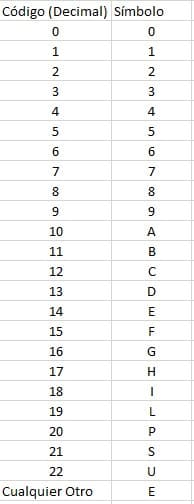
\includegraphics[scale = 0.5]{img/p1/alf.jpg}
		\caption{Alfabeto Decodificador 7 Segmentos}
		\label{fig:Alfabeto}
	\end{figure}
	
	Para representar el alfabeto anterior se diseño la tabla con las entradas y las salidas deseadas. 
	
	\begin{figure}[htb]
		\centering
		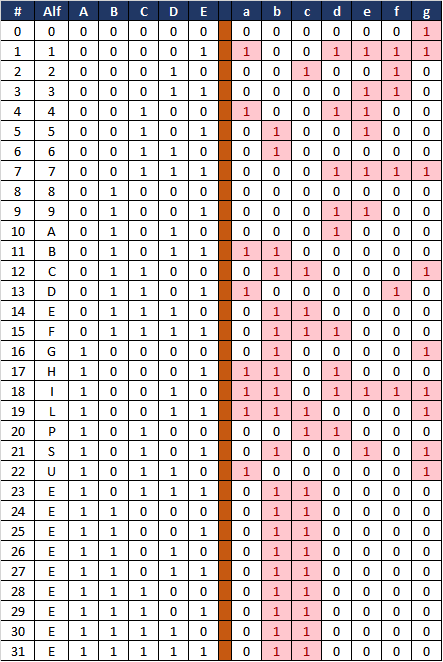
\includegraphics[scale = 0.5]{img/p1/alf_dis.png}
		\caption{Diseño Decodificador 7 Segmentos}
		\label{fig:disAlf}
	\end{figure}
	
	Posteriormente utilizando una herramienta online, se obtienen las funciones canónicas para las salidas que se esperan.
	
	\begin{figure}[htb]
		\centering
		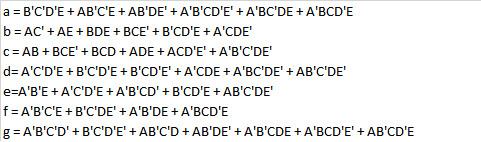
\includegraphics[scale = 0.8]{img/p1/funC1.png}
		\caption{Funciones Canónicas}
		\label{fig:funC}
	\end{figure}
	Las mismas en lenguaje de System Verilog tienen la siguiente sintaxis. 
	
	\begin{figure}[htb]
		\centering
		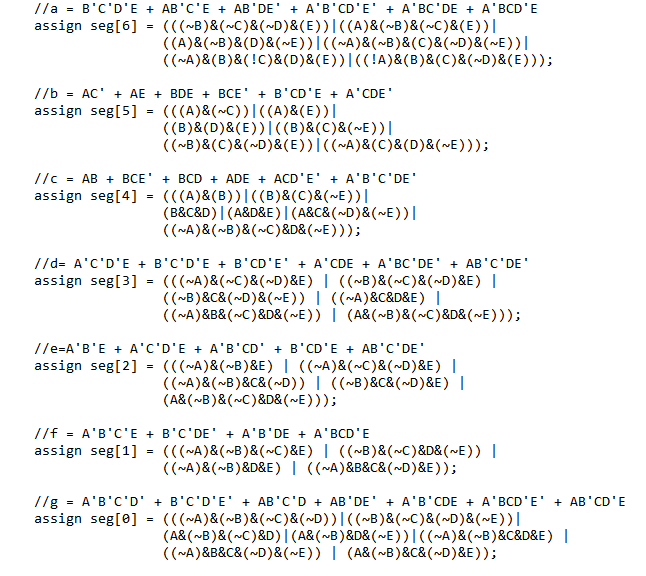
\includegraphics[scale = 0.5]{img/p1/funC1_SV.png}
		\caption{Funciones Canónicas en System Verilog}
		\label{fig:funCSV}
	\end{figure}
	
	\subsection{Análisis de Resultados}
	
	Para probar el funcionamiento del sistema, se utilizó un testbench, las pruebas se realizaron con las cadenas de bits 00000, 00001, 10000 y 01110, que según la Figura \ref{fig:disAlf} corresponden a 0, 1, G y E respectivamente. 
	\begin{figure}[htb]
		\centering
		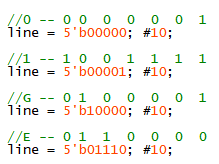
\includegraphics[scale = 0.8]{img/p1/tb1.png}
		\caption{Testbench Decodificador 7 Segmentos}
		\label{fig:tb1}
	\end{figure}
	
	Para el test realizado, y las salidas esperadas dadas las entradas mostradas se tienen los mostrados en la Figura \ref{fig:tb2}. 
	\begin{figure}[htb]
		\centering
		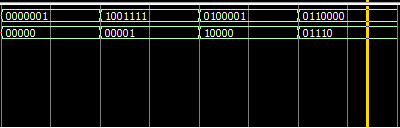
\includegraphics[scale = 0.8]{img/p1/tb2.png}
		\caption{Resultados de la Simulación}
		\label{fig:tb2}
	\end{figure}
	
	Con la simulación se puede apreciar que efectivamente, los valores obtenidos son los mostrados en la Tabla \ref{fig:disAlf}. 
	
	\section{Problema 2 : Sumador 5 bits}
	\subsection{Desarrollo y Resultados}
	
	Para la creación del sumador de 6 bits se utilizó la estructura básica del sumador de 1 bit, si conectamos sumadores de 1 bit en "serie", podremos obtener sumadores de N bits, en este caso se debe realizar un sumador de 6 bits, pero dadas las limitaciones de hardware de la FPGA se diseñó de 5 bits.
	
	De esta manera se utilizo el sumador de 1 bit para realizar la estructura básica, con un modelo de comportamiento. 
	
	\begin{figure}[htb]
		\centering
		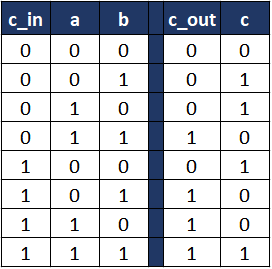
\includegraphics[scale = 0.8]{img/p2/sum6dis.png}
		\caption{Diseño de un Sumador de 1 bit}
		\label{fig:suma6dis}
	\end{figure}
	
	Los valores corresponden a: $c_{in}$, es el acarreo de entrada, a y b, son los valores que se desean sumar, c es el resultado de esta suma y $c_{out}$ es el acarreo de salida debido a un exceso de bits. Dados los datos de la Figura \ref{fig:suma6dis} se plantean las funciones canónicas que se aprecian en la Figura \ref{fig:suma6fc}.
	
	Estas funciones son escritas en VHDL, y utilizadas para hacer el modulo principal del programa. Mediante el acople de módulos se logra un sumador de 5 bits, con bandera de acarreo de salida. 
	
	\begin{figure}[htb]
		\centering
		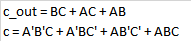
\includegraphics[scale = 0.8]{img/p2/fc6.png}
		\caption{Funciones Canónicas Sumador 1 bit}
		\label{fig:suma6fc}
	\end{figure}
	
	Además de ello, se diseña un modulo para representar los valores obtenidos en la FPGA. 
	\subsection{Análisis de Resultados}
	Al igual que en el problema anterior para analizar las entradas, se realiza en testbench. 
	
	Dada la cantidad de pares de sumas que se pueden realizar se van a analizar únicamente un par. 
	
	Primeramente tenemos 0 + 1, que en binario sería 00000 + 00001 y que como resultado se esperaría un 00001, para representar la salida de este programa se utilizaron 7 segmentos para representar cada uno de los bits de salida. 
	
	Si un 7 segmentos tiene como salida "1111001", simboliza una salida en alta, o un 1 lógico, pero si tiene como salida "1000000" simboliza una salida en bajo o un 0 lógico.  
	
	Por tanto la operación anterior debería dar como resultado el siguiente arreglo de 7 segmentos
	\begin{itemize}
		\item seg5 = 1000000
		\item seg4 = 1000000
		\item seg3 = 1000000
		\item seg2 = 1000000
		\item seg1 = 1000000
		\item seg0 = 1111001
	\end{itemize}
	A lo cual se obtuvo como resultados lo mostrado en la Figura \ref{fig:tbSum1}.
	
	\begin{figure}[htb]
		\centering
		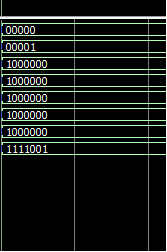
\includegraphics[scale = 0.8]{img/p2/tbS1.png}
		\caption{Test Bench Sumador 5 bits}
		\label{fig:tbSum1}
	\end{figure}
	El resultado es el esperado. 
	Las pruebas para demostrar el correcto funcionamiento se realizaron mediante pruebas físicas con la FPGA y mostraron los valores esperados. 
	
	
	\section{Problema 3 : Contador Parametrizable N bits }
	\subsection{Desarrollo y Resultados}
	Un contador es un circuito en el que sus salidas siguen una secuencia fija, que cuando acaba o es reiniciado vuelve a comenzar, el conteo puede ser sobre pulsos de reloj o bien pueden originarse por una fuente externa y ocurrir en intervalos fijos o aleatorios, además el número de salidas limita el número máximo que este puede contar. 
	Además cabe recalcar que los contadores son circuitos secuenciales por lo tanto se crean con flip-flops, que bien pueden ser de tipo D, T, J-K o también pueden crearse a partir de compuertas lógicas.
	Para este problema se solicita la creación de un contador asincrónico parametrizable de n bits, un contador de n bits puede contar desde 0 hasta $2^{n-1}$. El conteo se realiza mediante cambios en la entrada de los fip-flops, de manera que estos modifican sus estados dando lugar a un nuevo valor de salida, pero cuando la entrada no varía, los flip-flops conservan su estado presente.
	Existen dos grupos de contadores: sincrónicos y asincrónicos. Los contadores sincrónicos tienen un reloj interno, mientras que los asincrónicos no.
	
	\begin{figure}[htb]
		\centering
		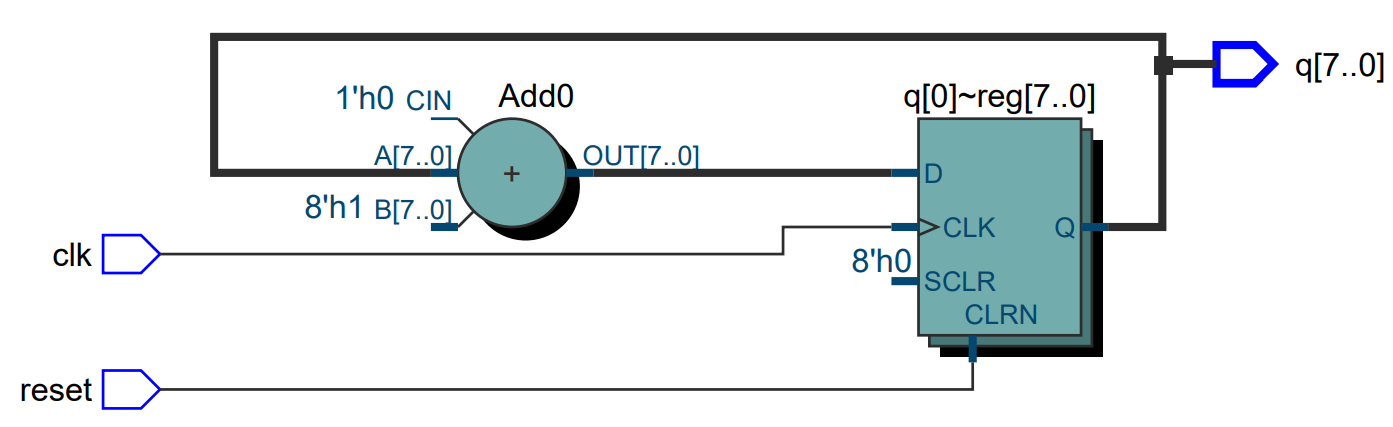
\includegraphics[scale = 0.22]{img/p3/counter8b.png}
		\caption{Contador 8 bits}
		\label{fig:counter8b}
	\end{figure}
	
	El contador desarrollado se puede observar en la Figura \ref{fig:counter8b}, este es un contador de parametrizable de 8 bits. Se desarrolló una tabla  que se muestra en la Figura \ref{fig:tncbd} con los números en binario y su representación decimal para un contador de 6 bits, aunque cabe destacar que funciona para el contador de 2 y 4 bits, únicamente tomando la cantidad de bits correspondiente.
	
	\begin{figure}[htb]
		\centering
		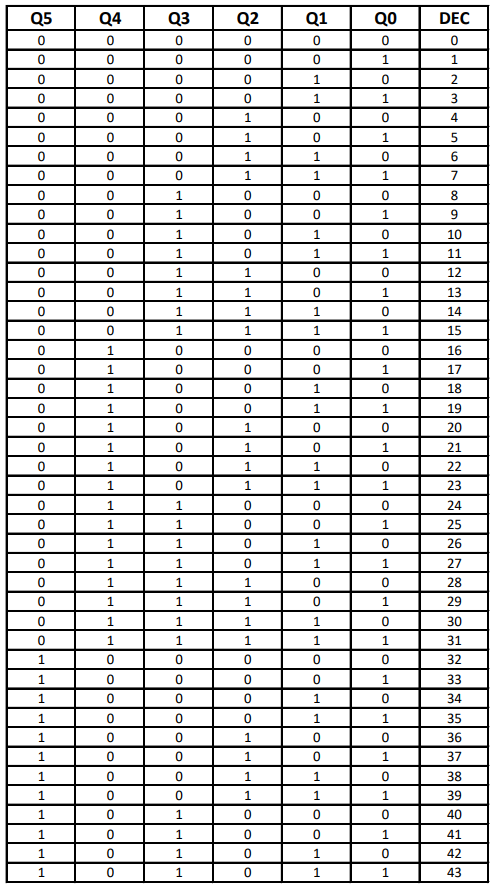
\includegraphics[scale = 0.6]{img/p3/tncbd.png}
		\caption{Tabla representación binaria y decimal de los números}
		\label{fig:tncbd}
	\end{figure}
	
	Posteriormente se realizó un testbench para contadores de 2, 4 y 6 bits para comprobar si los datos simulados corresponden a los teóricos, los resultados de este se encuentran en la Figura \ref{fig:rsc}.
	
	\begin{figure}[htb]
		\centering
		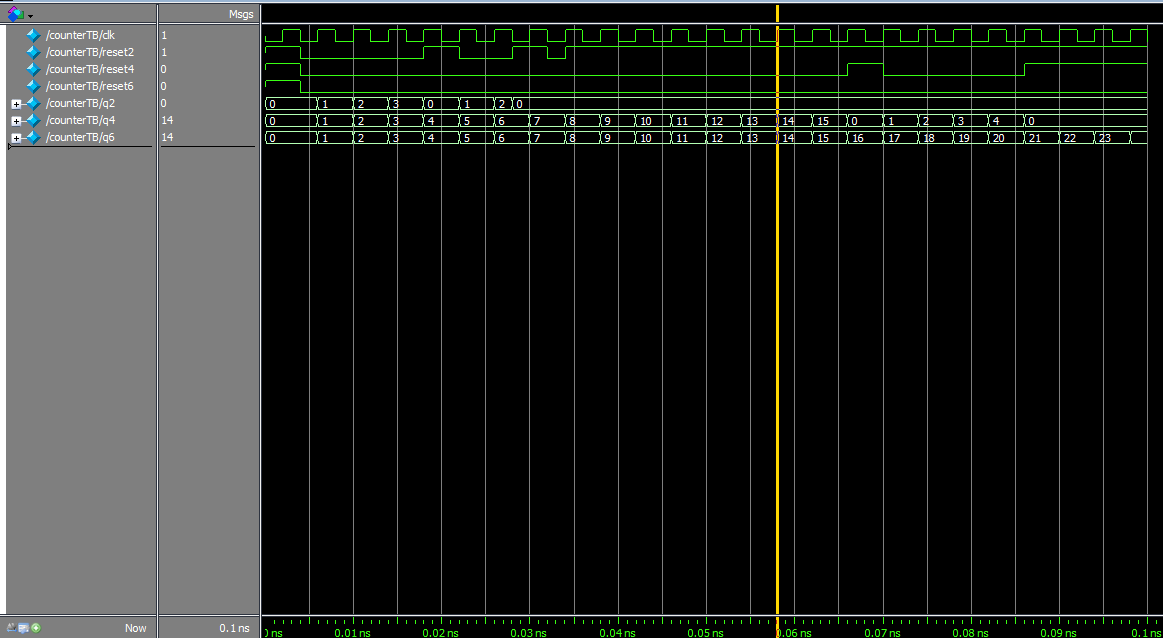
\includegraphics[scale = 0.25]{img/p3/rsc.png}
		\caption{Resultados obtenidos en el testbench}
		\label{fig:rsc}
	\end{figure}
	
	\subsection{Análisis de Resultados}
	
	Al igual que en los problemas anteriores se realizó un testbench para comprobar el correcto funcionamiento de las entradas y salidas de los contadores de 2, 4 y 6 bits, como se dislumbra en la Figura \ref{fig:rsc}.
	
	En la Figura \ref{fig:r1} se observa como al realizar el primer conteo los datos mostrados por la salidas de los contadores de 2, 4 y 6 bits corresponden con los previstos en la tabla de la Figura \ref{fig:tncbd}.
	
	\begin{figure}[htb]
		\centering
		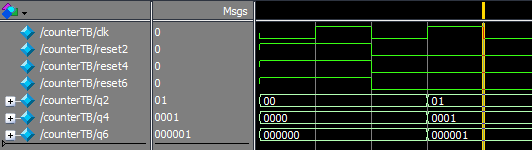
\includegraphics[scale = 0.4]{img/p3/r1.png}
		\caption{Resultados obtenidos en el testbench }
		\label{fig:r1}
	\end{figure}
	
	De la misma manera, en la Figura \ref{fig:rd} al cambiar la salida a números decimales como se observa en la Figura \ref{fig:r15} y contrastarlos con la tabla de la Figura \ref{fig:tncbd} se comprueba el correcto funcionamiento de los contadores de 4 y  bits, por lo que el desarrollo del contador parametrizable de n bits es correcto.
	
	\begin{figure}[htb]
		\centering
		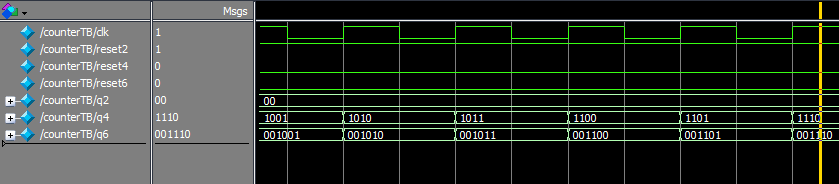
\includegraphics[scale = 0.3]{img/p3/rd.png}
		\caption{Resultados obtenidos en el testbench}
		\label{fig:rd}
	\end{figure}
	
	\begin{figure}[!htb]
		\centering
		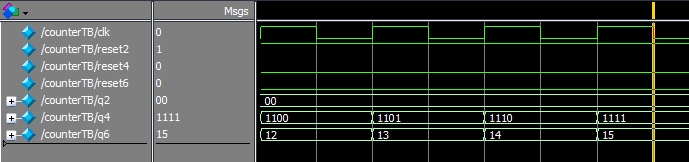
\includegraphics[scale = 0.4]{img/p3/r15.png}
		\caption{Resultados obtenidos en el testbench}
		\label{fig:r15}
	\end{figure}
	
	\section{Conclusiones}
	Para desarrollar soluciones debemos seguir una serie de pasos definidos para obtener resultados esperados, por lo general el inicio de un proyecto esta basado en la creación de un diseño o modelo que pueda representar el comportamiento que tendrá en un futuro la aplicación que estamos diseñando. En este caso para los problemas 1 y 2, se utilizó el modelo de comportamiento, para determinar la solución óptima que se adapte mejor a nuestras necesidades, mediante la creación de una tabla de verdad y la utilización de Mapas de Karnaugh. 
	
	Seguido de este paso, se procedió a realizar la solución que sigue los lineamientos de diseño, para esta fase, se tenia una idea del funcionamiento general de ambos programas, sin embargo, no fue hasta que se creo el "prototipo" de la aplicación que realmente se obtuvo lo deseado. 
	
	Por ende el utilizar las metodologías y herramientas de diseño, nos ayudan a utilizar eficientemente el tiempo, y por ende aumentar las ganancias que podamos percibir de nuestros proyectos.
	
	Realizar un testbench de auto-chequeo es de vital importancia para comprobar que el diseño implementado funciona correctamente o verificar errores y solucionarlos antes de realizar su conexión a la FPGA, permitiendo que encontrar dicho fallo sea menos engorroso.
	
	La FPGA es una herramienta útil en el diseño de módulos de hardware para circuitos simples, y para poder probar su viabilidad, y correcto funcionamiento, ya que el probarlos mediante un self-check sin duda alguna es importante, pero el poder comprobar su funcionamiento a nivel de hardware utilizando la FPGA representa mejor la importancia de los lenguajes de descripción de hardware y su infinidad de aplicaciones posibles mediante el uso de estas dos herramientas.
	
	\bibliographystyle{IEEEtran}
	\bibliography{myref}
	%https://jnjsite.com/vhdl-sumador-completo-de-1-bit/
	%https://www.intel.com/content/www/us/en/industrial-automation/programmable/applications/automation/overview.html 
\end{document}